\chapter{Implementation}
\label{sec:implementation}

This chapter describes the implementation of the kernels in \emph{C} (\cref{sub:impl_c}) and the wrappers
used to interface with them from \emph{Julia} (\cref{sub:impl_julia}). Additionally, \cref{sec:reproducibility}
describes how the code and experiments are managed and how to reproduce the results.

\section{Reproducibility}
\label{sec:reproducibility}

Before tackling the implementation of the kernels, it is important to discuss how the
code and its dependencies are managed to ensure reproducibility. This is addressed in
this section, where we describe the decisions taken to maximize reproducibility.

One of the main problems in machine learning research (and research in general) is the lack of
reproducibility of the results. There are a lot of factors that contribute to this, such as
the lack of documentation, the lack of code availability, the lack of standardization of
the experimental setup, etc. \cite{alstonBeginnerGuideConducting2021}. In this work, one of the main objectives is to make the
experimental setup as reproducible as possible.

\subsection{Dependency management}%
\label{sub:dependency_management}

\begin{wrapfigure}{r}{.40\textwidth}
    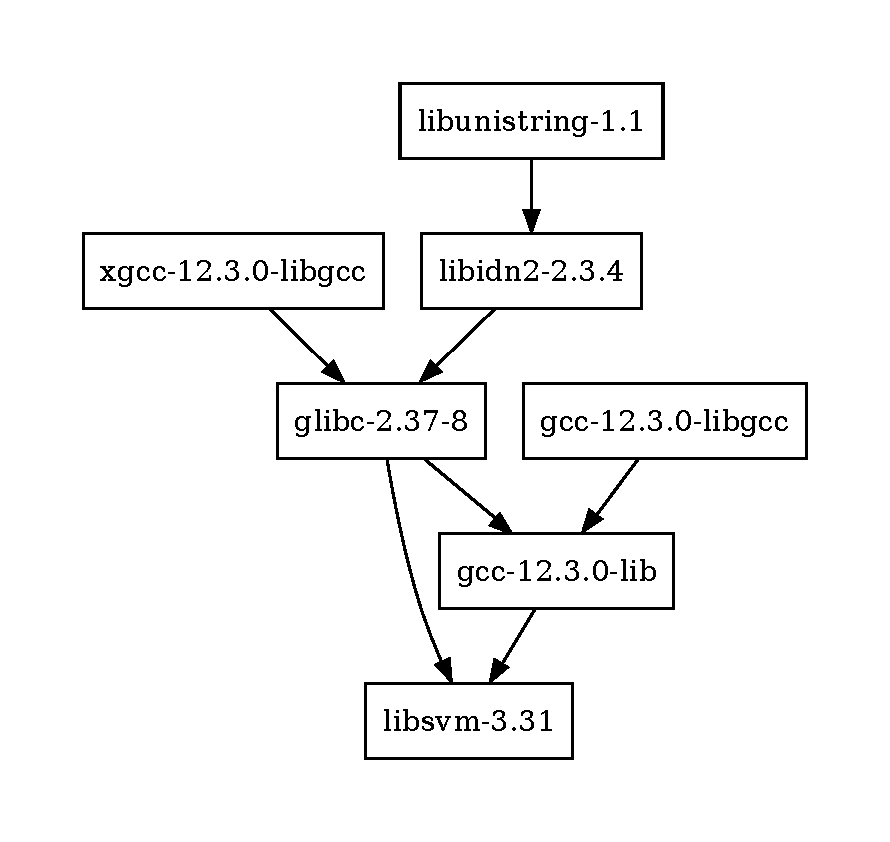
\includegraphics[width=.95\linewidth]{dependency_tree_libsvm}
    \caption{\emph{libsvm} runtime dependencies.}
    \label{fig:dependency_tree_libsvm}
\end{wrapfigure}

To manage the dependencies of the project, we use \emph{nix} \cite{NixNixOSReproducible}, a purely
functional package manager. \emph{Nix} allows us to keep a consistent environment across different
machines and operating systems. It keeps track of \emph{all} the system dependencies of the project
including all the libraries and tools (such as compilers, interpreters, etc.). For instance, with
\emph{nix} we can visualize the runtime dependency tree of the \emph{libsvm} library as shown in
\cref{fig:dependency_tree_libsvm}.

On the \emph{Julia} side, the dependencies are managed through \emph{Pkg} \cite{PkgJuliaLanguage}.
All this complexity is hidden from the user through \emph{direnv} \cite{DirenvUnclutterYoura}, which
automatically loads the environment when entering the project directory.

In summary, to reproduce the exact environment in which the experiments were run, the user only
needs to install \emph{nix} and \emph{direnv} and run \texttt{direnv allow} in the project directory.

All the datasets used are publicly available and are downloaded automatically by \emph{nix}. There
is a file \texttt{datasets.toml} which contains the URLs of the datasets and their checksums\footnote{The checksum uses \url{https://www.mankier.com/1/nix-hash}},
this guarantees that other users will know if the dataset has been modified.

\begin{listing}[htpb]
    \caption{Fragment of the \texttt{datasets.toml} file.}
    \label{lst:datasets_toml}
    \inputminted[firstline=29,lastline=35]{toml}{../datasets.toml}
\end{listing}

\subsection{Build system}

To build the project, we use \emph{Nix} as well. The \emph{Nix} build system is a declarative
build system which allows us to specify the exact build steps and dependencies of the project. Since
the build steps are sandboxed with no access to the system or the network, the build is guaranteed
to be reproducible as long as the process is deterministic (see \cref{sub:deterministic}).

\subsubsection{Determinism}
\label{sub:deterministic}

A deterministic build is a build that produces the same result given the same inputs. There are
many factors that can affect the result of a build, such as the time of the build, the use of random
numbers, race conditions, network access, etc.

To mitigate these factors, where possible, we use a fixed seed for the random number generator in
\emph{Julia} and set the \texttt{SOURCE\_DATE\_EPOCH} environment variable to a fixed date. The only
factor that we do not control is the execution order of different processes when running in parallel.
However, the multiple processes do not interact with each other in our case, so this should not
affect the result.

\subsection{Version control}

All versions of the code are stored in a \emph{git} repository hosted on GitHub. % TODO: link to repo
Additionally, all executions of experiments that generate data, store the commit hash of the
repository in which the code was run. This allows us to trace back the exact version of the code
used to generate the data. This is handled through the \texttt{DrWatson.jl} package \cite{datserisDrWatsonPerfectSidekick2020a}.

\subsection{Storing the results}

The \emph{DrWatson.jl} package also provides a mechanism to store the results of the experiments, in
which the results are serialized and stored in a \emph{JLD2} file (a julia-specific version of the \emph{HDF5} format).
Additionally, it stores several metadata fields such as the commit hash, the parameters used and other
information such as the computed performance metric or any other relevant information we may need.
The filename for each result saved is generated from the relevant parameters, which
allows checking whether a certain parameter configuration has already been computed and load it instead of recomputing it.

These \emph{JLD2} files contain the whole state of the trained machine models, which is useful to be able
to load the models and inspect them later. However, this also means that the files are quite large (several
hundred megabytes). For most analysis we are only interested in the performance metric of the model, so
along with the \emph{JLD2} files, we also store a \emph{CSV} file with the relevant information for each
model. This allows us to quickly load the results and perform analysis on them and, if necessary, we can load
the full model from the \emph{JLD2} file.
This workflow is illustrated in \cref{fig:experiment_flowchart}.

\begin{figure}[H]
    \begin{tikzpicture}
        % card with bullet points
        \node[draw, rectangle, minimum width=5cm, minimum height=3cm] (card) at (0,0) {};
        \node[anchor=north west] at (card.north west) {\textbf{Experiment\_1}};
        \node[anchor=north west] at ($(card.north west)+(0.2,-0.5)$) {- \texttt{sigma} = 0.1};
        \node[anchor=north west] at ($(card.north west)+(0.2,-1)$) {- \texttt{epsilon} = 0.5};
        \node[anchor=north west] at ($(card.north west)+(0.2,-1.5)$) {- \texttt{kernel} = \texttt{ArcSin}};
        \node[anchor=north west] at ($(card.north west)+(0.2,-2)$) {- \texttt{dataset} = \texttt{Triazines}};
        \node[anchor=north west] at ($(card.north west)+(0.4,-2.5)$) {\dots};

        \node (name) [below=of card] {\texttt{ex1\_sigma=0.1\_epsilon=0.5}\dots\texttt{.jld2}};
        \draw[-] (card) -- (name) node[midway, anchor=west] { filename};

        % if file exists, else

        \node[draw, diamond] (if) [below=of name] {Exists?};
        \draw[->] (name) -- (if);
        \node[draw, rectangle, rounded corners] (load) [left =of if] {Load};
        \node[draw, rectangle, rounded corners] (run) [right=of if] {Run};
        \draw[->] (if) -- (load) node[midway, anchor=south] {yes};
        \draw[->] (if) -- (run) node[midway, anchor=south ] {no};

        \coordinate [right=of name] (nameright) {};
        \node (csv) [right=of nameright] {\texttt{ex1\_results.csv}};

        \draw[-] (run.east) -| (nameright) node[midway, anchor=south west] {save};
        \draw[->] (nameright) |- (name);

        \draw[->] (run.east) -| (csv.south) node[midway, anchor=south west] {append};
    \end{tikzpicture}
    \caption{Flowchart of the experiment execution and results storage.}
    \label{fig:experiment_flowchart}
\end{figure}

\subsection{Running the experiments}

All the relevant code to the experiments is contained in the \texttt{src} directory and scripts
that run the experiments are in the \texttt{scripts} directory and named after their corresponding
experiment. To run an experiment, we can simply call the corresponding \emph{Julia} script:
\mintinline{bash}{julia scripts/experiment_1.jl}. The dependencies can be installed automatically
using \emph{Nix} and \emph{direnv} as described in \cref{sub:dependency_management}, with
\mintinline{bash}{direnv allow} or \mintinline{bash}{nix develop}.

Additionally, the \mintinline{bash}{nix build} command can be used to build the document
and a tarball with the datasets.

\section{Extending \texttt{libsvm}}%
\label{sub:impl_c}

\emph{libsvm} is a C library developed by \textcite{CC01a} under BSD-3 license which implements the
Support Vector Machine (SVM) algorithm. The library is the de facto standard for SVM implementations in
the machine learning community, being used by many other libraries and frameworks such as
Python's sklearn~\cite{ScikitlearnScikitlearn2023} or R's e1071~\cite{meyer[autE1071MiscFunctions2023}.

Out of the box, \emph{libsvm} supports using the built-in kernels: linear, polynomial,
radial basis function (RBF) and sigmoid. Additionally, it can use precomputed kernel matrices
by setting the kernel type to \texttt{PRECOMPUTED} and passing the kernel matrix as the
training data.

\subsection{Adding the kernels}

For our purposes, we want to extend the library by adding our own kernels. To do so, we
need to modify the library source by adding the corresponding kernel functions. The kernel
type is specified through an \texttt{enum}, so we can add our own kernels to it and extend the
switch statements in the code to handle them. The modification is thus quite straightforward.
\cite{arquemartinezDissenyImplementacioEstudi2021}

From there, we have to implement the kernel functions themselves. Surprisingly at first,
the kernel functions are duplicated in the code for each kernel type:
\texttt{k\_function} and \texttt{kernel\_function}. The former is used for the training
phase and the latter for the prediction phase. This is explained in the \emph{libsvm}'s
FAQ \cite{LIBSVMFAQ}:

For the RBF kernel, Instead of doing $\exp\left(-\gamma\|x_i - x_j\|^2\right)$, it computes
$\exp\bigl(-\gamma(\|x_i\|^2 - 2x_i^Tx_j + \|x_j\|^2)\bigr)$, and by precomputing
$\|x_i\|^2$ for all $x_i$ in the beginning, the number of operations is reduced from
$3n$ to $2n$. This same optimization can be applied to our kernels.

The first step, is to add the new kernel types to the \texttt{enum} in \texttt{svm.h} as
shown in \cref{lst:svm_h_enum}.
\begin{listing}[H]
    \caption{Modified Enum definition from \texttt{svm.h}}
    \label{lst:svm_h_enum}
\begin{minted}{C}
enum { LINEAR, POLY, RBF, SIGMOID, PRECOMPUTED, ASIN, ASIN_NORM, ACOS_0, ACOS_1, ACOS_2}; /* kernel_type */
\end{minted}
\end{listing}
Then, we add the corresponding cases to the switch statements in \texttt{svm.cpp} for both
\texttt{k\_function} and \texttt{kernel\_function} as shown in \cref{lst:kernel_function}.
The prediction case (\texttt{k\_function}) is not shown for brevity, but it is similar
to the training case. The only difference is the use of the precomputed dot
product of $x_i$ with itself (\texttt{x\_square}),
which is passed as a parameter to the kernel function (See \cref{lst:svm_cpp_k_function} in the appendix)

In order to avoid code duplication and make the code more readable, we added the helper functions for
the \texttt{asin} kernel shown in \cref{lst:svm_cpp_helper}.

Another minor optimization for the \texttt{asin} kernel, instead of computing $\frac{1}{2\sigma_w^2}$ every time as
shown in the original \cref{eq:kernel_asin}, we define
$\gamma = \frac{1}{2\sigma_w^2}$ and pass it as a parameter to the kernel function.

\begin{listing}
    \caption{Helper functions for the asin kernel (\texttt{svm.cpp})}
    \label{lst:svm_cpp_helper}
\begin{minted}{C}
// Passing x_square and y_square as parameters, we can avoid computing them again
// every time we call the kernel function
static inline double asin_elm(const svm_node *x, const svm_node *y, const double x_square, const double y_square, const double gamma) {
    return asin((1.0 + dot(x, y))/sqrt( (gamma + 1.0 + x_square)* (gamma + 1.0 + y_square)) );
};

// Fallback method used in prediction
static inline double asin_elm(const svm_node *x, const svm_node *y, const double gamma) {
    return asin_elm(x, y, dot(x), dot(y), gamma);
}

// AsinELM with x=y, for faster computation, we don't need to compute the sqrt
static inline double asin_elm_equal(const double x_square, const double gamma) {
    const double x_square_plus_one = 1.0 + x_square;
    return asin(x_square_plus_one/(gamma + x_square_plus_one));
}
\end{minted}
\end{listing}

\begin{listing}
    \caption{Implementation of the kernels in \texttt{svm.cpp} for the training phase. Notice the use of
        \texttt{x\_square} to avoid computing the dot product of $x$ with itself every time it is needed.
    }
    \label{lst:kernel_function}
\begin{minted}{C}
double kernel_asin(int i, int j) const
{
    return M_2_PI*asin_elm(x[i], x[j], x_square[i], x_square[j], gamma);
}
double kernel_asin_norm(int i, int j) const
{
    return asin_elm(x[i], x[j], x_square[i], x_square[j], gamma)/sqrt(
        asin_elm_equal(x_square[i], gamma)*asin_elm_equal(x_square[j], gamma)
    );
}
double kernel_acos_0(int i, int j) const
{
    return 1.0 - M_1_PI*acos(dot(x[i], x[j])/sqrt(x_square[i]*x_square[j]));
}
double kernel_acos_1(int i, int j) const
{
    const double x2y2 = x_square[i]*x_square[j];
    const double xy = sqrt(x2y2);
    const double cos_theta = dot(x[i], x[j])/xy;
    const double theta = acos(cos_theta);
    return M_1_PI*xy*(sin(theta) + (M_PI - theta)*cos_theta);
}
double kernel_acos_2(int i, int j) const
{
    const double x2y2 = x_square[i]*x_square[j];
    const double sqrt_x2y2 = sqrt(x2y2);
    const double dot_xy = dot(x[i], x[j]);
    const double cos_theta = dot_xy/sqrt_x2y2;
    const double cos2_theta = dot_xy*dot_xy/x2y2;
    const double theta = acos(cos_theta);
    return M_1_PI*x2y2*(3*sin(theta)*cos_theta + (M_PI - theta)*(1 + 2*cos2_theta));
}
\end{minted}
\end{listing}

\subsection{Controlling the number of iterations}

One metric which we wanted to measure was the number of iterations the SVM algorithm took
and have the possibility to stop it early. To do so, \emph{libsvm} only provides a
\texttt{tolerance} parameter for the stopping criterion. However, in \emph{sklearn}
they provide a \texttt{max\_iter} parameter\footnote{\url{https://github.com/scikit-learn/scikit-learn/pull/1184}}
which is the maximum number of iterations
and also report the number of iterations the algorithm took
\footnote{\url{https://github.com/scikit-learn/scikit-learn/pull/21408}}.
This is accomplished by
using a modified version of \emph{libsvm}. Since we are modifying the library as well,
we added the same functionality to our modified version

\section{Julia}%
\label{sub:impl_julia}

\emph{Julia} \cite{bezanson2017julia} is a high-level, high-performance dynamic programming language
which is designed from the ground up to be fast, expressive, and easy to write. Its aim is to provide
the ease of use of a scripting language such as Python while being as fast as a compiled language
such as C. In particular, \emph{BinaryBuilder.jl} \cite{JLLPackagesBinaryBuilder} allows reproducible
cross-platform compilation of 3rd party libraries for different platforms and architectures.
This is used throughout the Julia ecosystem to provide binary dependencies for packages,
for example, \emph{libsvm} is provided by the \emph{libsvm\_jll} package \cite{LibsvmJllJl2022}.
This makes it very easy to change the \emph{libsvm} library used by a package by simply changing
the dependency to our modified \emph{libsvm\_jll} package.

For this reasons, and the fact that there is a large and growing number of machine learning
packages in Julia, we decided to interface our modified \emph{libsvm} library with Julia.

\subsection{libsvm\_jll}

As mentioned before, the \emph{libsvm\_jll} package is a compiled version of the \emph{libsvm} C library
compiled through \emph{BinaryBuilder.jl}. This so-called \emph{Julia Link Library} (JLL) package
is not much different from a regular system library, except that its dependencies are dynamically
linked to other JLL packages.

For our implementation, we used the original recipe from \textcite{LibsvmJllJl2022} and modified it
to use our modified \emph{libsvm} source code.

\subsection{LIBSVM.jl}

The \emph{LIBSVM.jl} package \cite{LIBSVMJl2023} is a Julia wrapper for the \emph{libsvm} library which
provides a high-level interface to the library. It uses the artifacts generated by the \emph{libsvm\_jll}
package and provides the translation between Julia types and the C types used by the library.

\subsubsection{Adding the kernels}

The kernels can be added by extending the \texttt{Kernel} \texttt{enum} in Julia to reflect the
\texttt{enum} in the C library.
\begin{listing}[H]
\begin{minted}{julia}
module kernel
@enum KERNEL Linear Polynomial RadialBasis Sigmoid Precomputed Asin AsinNorm Acos0 Acos1 Acos2
end
\end{minted}
\caption{Julia \texttt{enum} definition for the kernels, equivalent to the C definition in \cref{lst:svm_h_enum}.}
\label{lst:kernel_enum_julia}
\end{listing}

Technically, this is the only change needed to add the kernels to the library, since the
\emph{C} library has the kernel functions implemented and selects them based on the kernel type enum.

\subsubsection{Adding the number of iterations}

The modification of the number of iterations is a little more involved and requires modifying the
\texttt{SVMModel} and \texttt{SVMParameter} types to store the number of iterations as well
as properly copying the values from the C pointer into Julia object. In order to test that
this was properly implemented, we added a test set to \emph{LIBSVM.jl}. The tests
validate that the number of iterations copied from the C pointer is the same as the one
returned by the \emph{libsvm} library and that \texttt{max\_iter} is respected.

\subsubsection{libsvm 3.31}

The version of \emph{libsvm} used by \emph{LIBSVM.jl} is 3.25. It has not been updated to the
newest version 3.31, since it breaks the API by adding the option of
probability density estimation. Again, we worked around this by modifying the library to properly
handle the new API (this change will be upstreamed to \emph{LIBSVM.jl}). % TODO: link to PR

\subsection{MLJ}

\emph{MLJ} \cite{blaomMLJJuliaPackage2020} is a machine learning framework for Julia which provides a common interface
for many machine learning packages. It is the equivalent of \emph{scikit-learn} in Python. It provides
an interface to \emph{LIBSVM} through the \emph{MLJLIBSVMInterface.jl} package. By modifiying the latter
package to include the \texttt{max\_iter} parameter, we can use it in \emph{MLJ}.

From this point, we can use all the functionality provided by \emph{MLJ} to train, evaluate,
tune and visualize our SVM models with flexibility and ease.

\Cref{fig:julia_libsvm_deps} shows the relationship between the packages and how the
libraries interface with each other.

\begin{figure}[H]
\begin{tikzpicture}[
    box/.style={draw, rectangle, minimum width=1cm, minimum height=1cm},
    C/.style={fill=lightgray},
    Julia/.style={fill=lime!70},
    JLL/.style={fill=orange!50},
    ]
    \node[box,C] (libsvm) at (0,0) {libsvm};
    \node[box,JLL,below=of libsvm] (libsvm_jll) {libsvm\_jll};
    \node[box,Julia,right=of libsvm_jll] (LIBSVM) {LIBSVM.jl};
    \node[box,Julia,right=of LIBSVM] (MLJLIBSVMInterface) {MLJLIBSVMInterface.jl};
    \node[box,Julia,below=of MLJLIBSVMInterface] (MLJ) {MLJ.jl};

    \draw[->] (libsvm) -- (libsvm_jll) node[midway, anchor=west,color=lime!60!black] {build\_tarballs.jl};
    \draw[->] (libsvm_jll) -- (LIBSVM);
    \draw[->] (LIBSVM) -- (MLJLIBSVMInterface);
    \draw[->] (MLJLIBSVMInterface) -- (MLJ);

    % Color Legend
    \matrix [draw,right] at ($(current bounding box.east)+(0.5,0)$) {
      \node [C,label=right:C] {}; \\
      \node [JLL,label=right:Julia Link Library] {}; \\
      \node [Julia,label=right:Julia] {}; \\
    };

\end{tikzpicture}
\caption{Dependency graph of Julia packages exposing the libsvm library API.}
\label{fig:julia_libsvm_deps}
\end{figure}

The forked versions of the libraries discussed in this section can be found in the following
repositories:
\begin{itemize}
    \item \url{https://github.com/LeixB/libsvm}
    \item \url{https://github.com/Leixb/build\_tarballs\_libsvm\_jll}
    \item \url{https://github.com/Leixb/libsvm\_jll.jl}
    \item \url{https://github.com/LeixB/LIBSVM.jl}
    \item \url{https://github.com/LeixB/MLJLIBSVMInterface.jl}
\end{itemize}

% \subsection{Memoization}
% TODO: Check if memoization if worth it or if we can do it manually in a more
% sensible way.

